\begin{figure}[htbp]
\centering
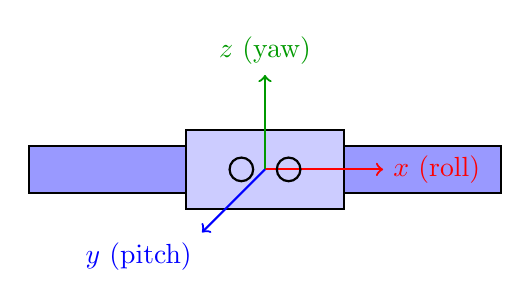
\begin{tikzpicture}
    % Satellite body
    \draw[thick, fill=blue!20] (-1,-0.5) rectangle (1,0.5);

    % Solar panels
    \draw[thick, fill=blue!40] (-3,-0.3) rectangle (-1,0.3);
    \draw[thick, fill=blue!40] (1,-0.3) rectangle (3,0.3);

    % Body axes
    \draw[->, thick, red] (0,0) -- (1.5,0) node[right] {$x$ (roll)};
    \draw[->, thick, green!60!black] (0,0) -- (0,1.2) node[above] {$z$ (yaw)};
    \draw[->, thick, blue] (0,0) -- (-0.8,-0.8) node[below left] {$y$ (pitch)};

    % Reaction wheels (symbolic)
    \draw[thick] (0.3,0) circle (0.15);
    \draw[thick] (-0.3,0) circle (0.15);
\end{tikzpicture}
\caption{Satellite with body-fixed axes.}
\label{fig:satellite}
\end{figure}
